\documentclass[11pt]{article}
\usepackage[letterpaper, margin=0.8in]{geometry}
\usepackage{amsmath}
\usepackage{amssymb}
\usepackage{wrapfig}
\usepackage[makeroom]{cancel}
\usepackage{bbm}
\usepackage{booktabs}
\usepackage{float}
\usepackage{array}
\usepackage{bm}
\usepackage{enumerate}
\usepackage{amsfonts} 
\usepackage{color}
\usepackage{algorithm}
\usepackage[noend]{algpseudocode}
\usepackage{hyperref}
\usepackage{xcolor}
\usepackage{hyperref}
\usepackage{newfloat}
\usepackage{graphicx}
\usepackage{caption}
\usepackage{fancyhdr}
\usepackage{bbm}
\usepackage[overload]{empheq}
\newcommand{\IF}{\text{if }}
\newcommand{\norm}[1]{\left\lVert#1\right\rVert}
\def\changemargin#1#2{\list{}{\rightmargin#2\leftmargin#1}\item[]}
\let\endchangemargin=\endlist 
\newcommand\inner[2]{\langle #1, #2 \rangle}
\pagestyle{fancy}
\fancyhf{}
\captionsetup[figure]{labelfont={bf},name={Figure}}
\captionsetup[table]{labelfont={bf},name={Table}}
\rhead{\thepage}
\DeclareMathOperator*{\argmin}{\arg\!\min}
\DeclareMathOperator*{\argmax}{\arg\!\max}

\title{Spectral Clustering : what to do after getting the similarity matrix $S$}

\begin{document}
\noindent While trying to figure out the role of Laplacian matrix and its potential benefit of including it in the optimization goal, I realized that the reason I feel lost and disorganized at this stage is not because of the optimization goal but because of spectral clustering. So far I have been testing baseline spectral clustering, straight-up kmeans, and t-sne for each algorithm's output similarity matrices, and the frustrating part is that for each optimization goal, different clustering methods show the best performance. (For example, nuclear norm generally performs better with t-SNE, but when rank is controlled through hard-thresholding without convex relaxation, baseline spectral clustering works better.) Moreover, the performance is better in one method for some data sets but worse for other data sets. This is why performance comparison often feels inconclusive - even with the same similarity matrix, performance is different (not by much in terms of evaluation measure like NMI, but in terms of ordering - which performs better?).\\

\noindent I organized four methods below. However, there are more than just 4: within each method, I can use (a) binary adjacency matrix or continuous weighted edge matrix (if using binary adjacency matrix, knn or thresholding? how many k for knn? which threshold for thresholding?), (b) normalized Laplacian or unnormalized Laplacian, and (c) kmeans on entire matrix or kmeans on the matrix of only k eigenvectors. This exponentially increases the number of tests I need to conduct, and it has been difficult to make a consistent conclusion of which is better than which.\\

\noindent My current thought is to decrease the number of tests by trying only the conventionally “better” method. For example, we can only use normalized Laplacian and not unnormalized one, and use normalized spectral clustering instead of straight-up kmeans, even if this decision leads to poor performance for some optimization goals and for some data sets.\\

\noindent And of course on top of all this, we need to decide the kernel parameters. There are too many things we can play with, and I'm overwhelmed.


\section*{Kmeans}
\begin{itemize}
\item start with similarity matirx $S$
\item kmeans clustering on $S$, or on the first $k$ eigenvalues of $S$
\end{itemize}

\section*{Baseline Spectral Clustering}

\begin{itemize}
\item start with similarity matrix $S$
\item construct adjacency matrix $A$ with binary 0/1 elements using hard thresholding or knn
\item Get Laplacian matrix $L$, either normalized $L = (D^{-1/2} (D-A) D^{-1/2})$ or unnormalized $L = (D-A)$.
\item Get the matrix of eigenvectors $U$ of $L$ corresponding to the $k$ smallest eigenvalues. 
\item kmeans clustering on $U$
\end{itemize}


\section*{Normalized spectral clustering by Ng et al (2002)}
\begin{itemize}
\item start with similarity matrix $S$
\item construct a similarity graph using weighted (or unweighted / binary) adjacency matrix
\item construct normalized Laplacian matrix $L$
\item compute the first $k$ eigenvectors of $L$
\item construct matrix $T$ by normalizing the rows to norm 1
\item kmeans clustering on $T$
\end{itemize}

\section*{t-SNE (2008)}
\begin{itemize}
\item start with similarity matrix $S$
\item compute Laplacian $L$ from similarity matrix $S$
\item use initial solution $\mathcal{Y}^{(0)}$ as the last $k$ eigenvectors of the Laplacian matrix $L$
\item for $t = 1$ to $T$, compute low dimensional affinities $q_{ij}$, compute gradient, and update $\mathcal{Y}_t$
$$\mathcal{Y}^{(t)} = \mathcal{Y}^{(t-1)} + \eta \frac{\partial C}{\partial \mathcal{Y}} + \alpha (t) (\mathcal{Y}^{(t-1)} - \mathcal{Y}^{(t-2)})$$
\end{itemize}

\clearpage

\noindent 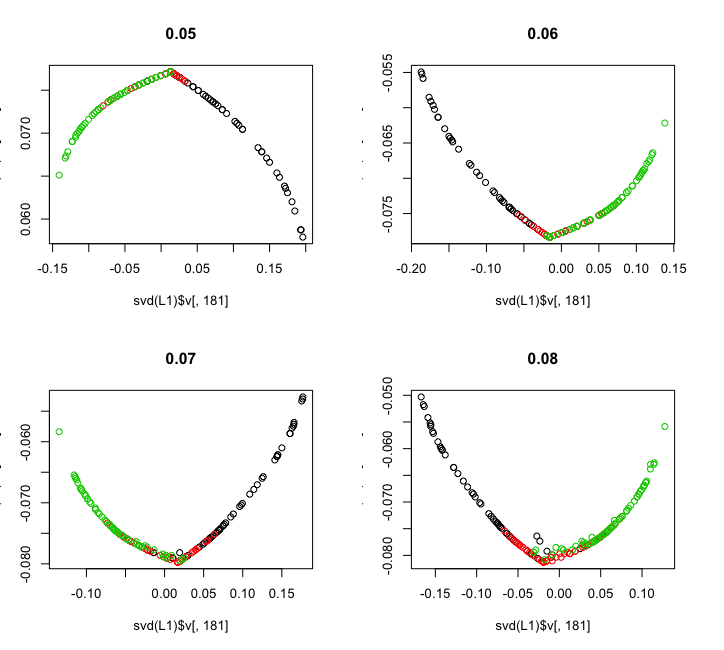
\includegraphics[width=0.48\textwidth]{thresh1.png}
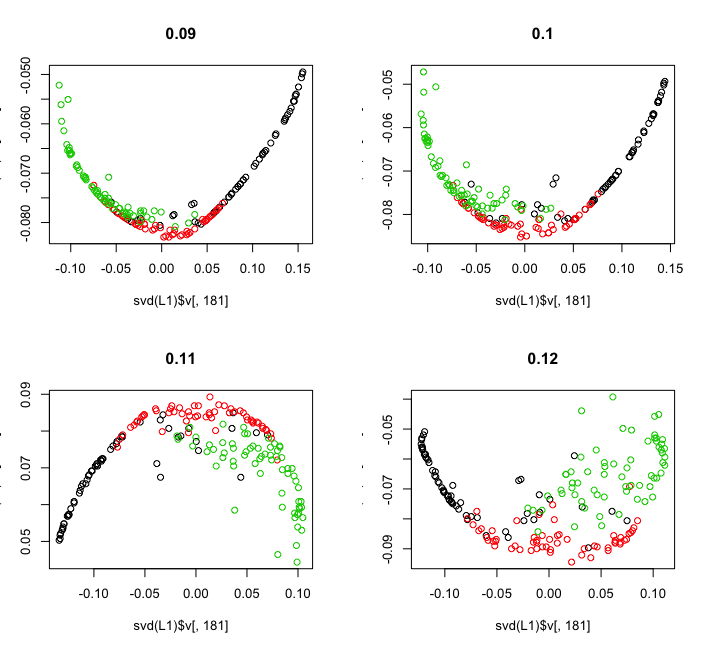
\includegraphics[width=0.48\textwidth]{thresh2.png}\\
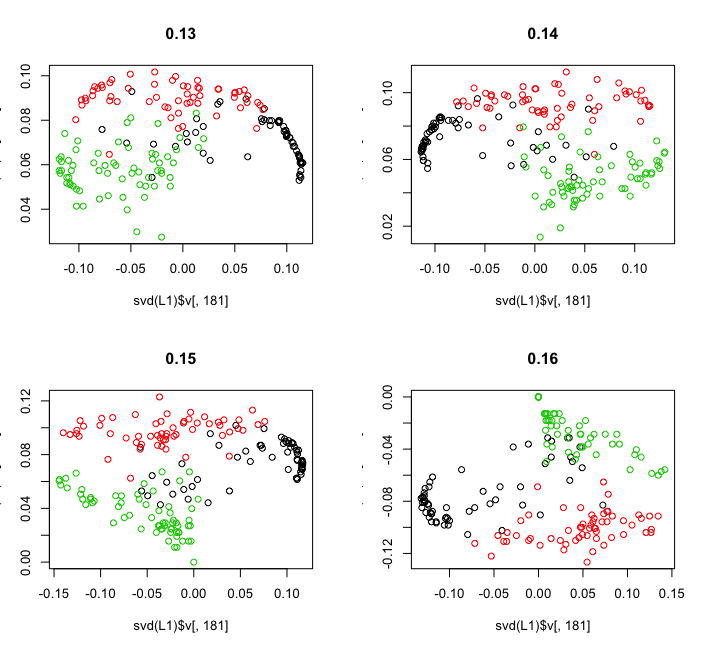
\includegraphics[width=0.48\textwidth]{thresh3.png}
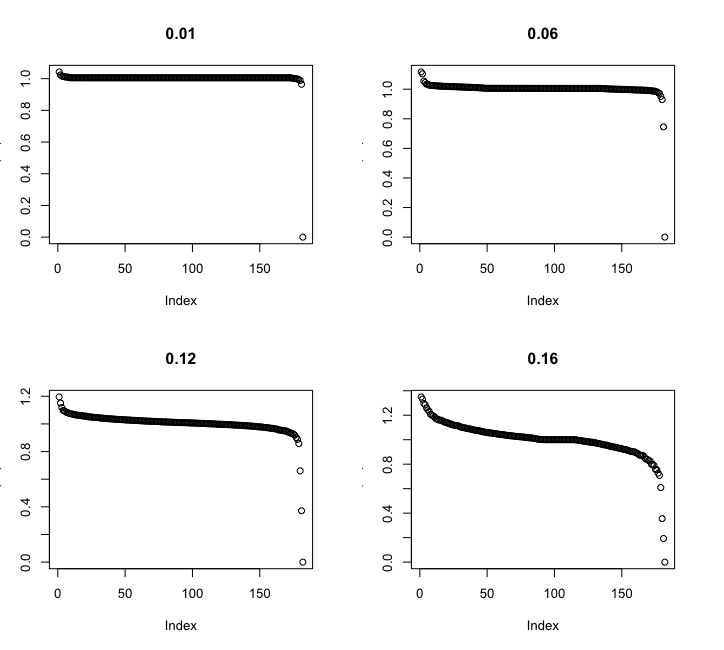
\includegraphics[width=0.48\textwidth]{sv.png}


\clearpage
\noindent 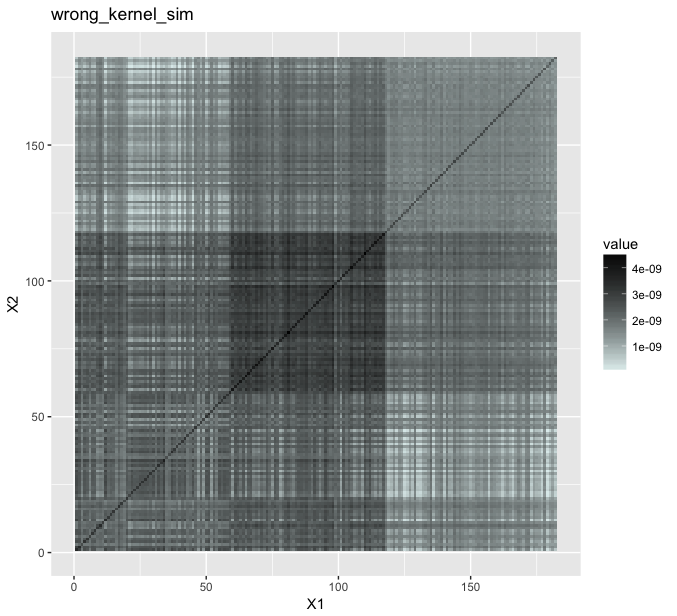
\includegraphics[width=0.48\textwidth]{wrongkernelsim.png}
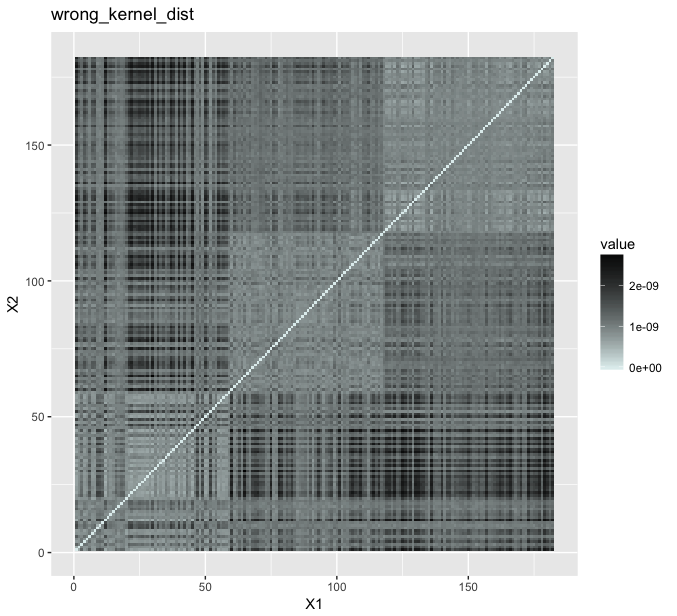
\includegraphics[width=0.48\textwidth]{wrongkerneldist.png}\\
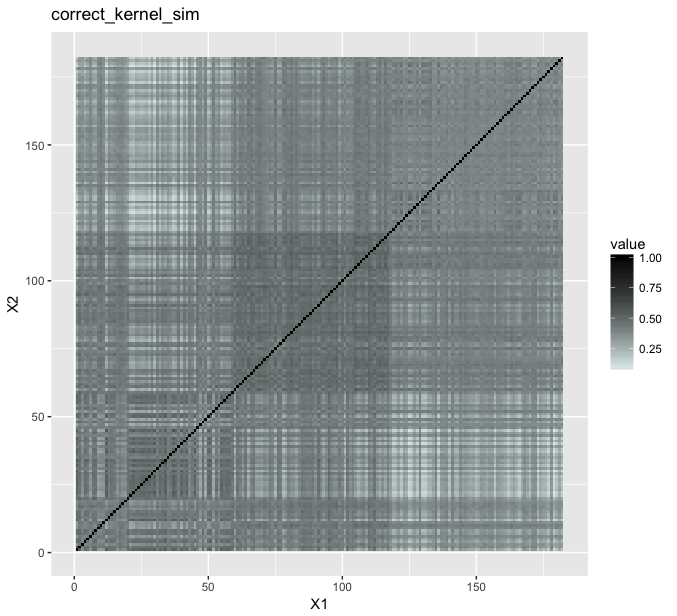
\includegraphics[width=0.48\textwidth]{correctkernelsim.png}
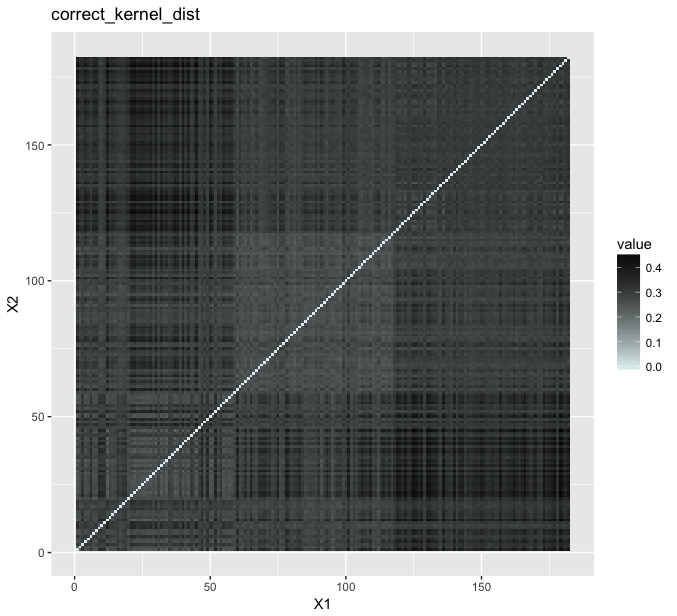
\includegraphics[width=0.48\textwidth]{correctkerneldist.png}




\end{document}







